\documentclass[letterpaper, 10 pt, conference]{ieeeconf}  % Comment this line out if you need a4paper
%\documentclass[a4paper, 10pt, conference]{ieeeconf}      % Use this line for a4 paper
\IEEEoverridecommandlockouts                              % This command is only needed if 
                                                          % you want to use the \thanks command
\overrideIEEEmargins                                      % Needed to meet printer requirements.

\usepackage[pdftex]{graphicx}
\usepackage{algpseudocode}
\usepackage[noadjust]{cite}

\title{\LARGE \bf
  Reactive Path Planning with Pedestrains for Autonomous Driving
}

\author{
  Robert G. Cofield $^{1}$,
  Rakesh Gupta $^{2}$,
  Ambarish Goswami $^{3}$,
  and
  David Bevly $^{4}$
  \thanks{
    * This work was performed at Honda Research Institute USA.
  }
  \thanks{
    $^{1}$ Robert G. Cofield is a graduate researcher at Auburn University's GPS \& Vehicle Dynamics Laboratory.
  }
  \thanks{
    $^{2}$ Rakesh Gupta ...
  }
  \thanks{
    $^{3}$ Ambarish Goswami ... 
  }
  \thanks{
    $^{4}$ David Bevly ...
  }
}


%%%%%%%%%%%%%%%%%%%%%%%%%%%%%%%%%%%%%%%%%%%%%%%%%%%%%%%%%%%%%%%%%%%%%%%%%%%%%%%%
%%%%%%%%%%%%%%%%%%%%%%%%%%%%%%%%%%%%%%%%%%%%%%%%%%%%%%%%%%%%%%%%%%%%%%%%%%%%%%%%
%%%%%%%%%%%%%%%%%%%%%%%%%%%%%%%%%%%%%%%%%%%%%%%%%%%%%%%%%%%%%%%%%%%%%%%%%%%%%%%%

\begin{document}

\maketitle
\thispagestyle{empty}
\pagestyle{empty}

%%%%%%%%%%%%%%%%%%%%%%%%%%%%%%%%%%%%%%%%%%%%%%%%%%%%%%%%%%%%%%%%%%%%%%%%%%%%%%%%
\begin{abstract}

Minimize of navigation time from origin to the destination implies two tasks that can be carried out sequentially or in parallel. First is Path Planning which involves computation of the shortest path. Second task is Velocity Planning (or Trajectory Generation) which involves the computation of the fastest velocity profile that is smooth and comfortable for the human occupant.

For human comfort, it is widely believed that high levels of jerk (time derivative of acceleration) and high acceleration/velocity values are prime contributors to ride discomfort. A lot of work has been performed on optimizing these constraints for highways and country roads ~\cite{ziegler14,bahram15,xu12,CHEB15CI}. Some preliminary work on optimizing these constraints on urban roads has been done ~\cite{Rastelli14,Li15} but they do not consider reactive behavior such as responding to pedestrians or other dynamic objects in the scene. On the other hand systems that find and plan paths around pedestrians, stop for them, or produce a warning ~\cite{pradalier05,benenson06,gu14,mogelmose15,johnson13} do not work as part of an integrated system that can navigate urban roads. In this paper, we describe an trajectory generation system that satisfies these constraints for human comfort as well is reactive to presence of pedestrians on the road.


\end{abstract}
%%%%%%%%%%%%%%%%%%%%%%%%%%%%%%%%%%%%%%%%%%%%%%%%%%%%%%%%%%%%%%%%%%%%%%%%%%%%%%%%

%%%%%%%%%%%%%%%%%%%%%%%%%%%%%%%%%%%%%%%%%%%%%%%%%%%%%%%%%%%%%%%%%%%%%%%%%%%%%%%%
\section{Introduction} \label{sec:introduction}

In this paper we present an autonomy framework for pedestrian aware ground vehicles. We describe the objective and architecture.
Then we describe other subsystems that our system needs to work with, and planned stops. We then describe
reactivity to pedestrians in the environment by extending the trajectory planner. We then summarize and discuss future extensions.
Some work has been done for reacting to pedestrians such as by Singapore groups but it has been done
at very low speeds (5 miles/hour). There has also been some work in simulating vehicles and modeling
uncertainty, but pedestrians are less predictable than cars and can appear suddenly on the road 
(when someone is jaywalking for example). 

Our objective is to travel autonomously from start to destination while honoring traffic laws and avoiding pedestrians on the roadway. We assume that there is no other traffic on the roadway. Desired behavior from the car includes following traffic laws at the intersections such as stop signs. At stop signs the car should stop and wait for an appropriate amount of time. It should also react to pedestrians on the road - at intersections as well as on the road. If pedestrians are not on the road they should be ignored by the autonomous cars. Further the pedestrians can be static or moving. The car should stop, slow down and circum-navigate around pedestrians when appropriate.


In urban scenarios we need to handle intersections, turns in the road and planned stops due 
to stop signs (that have already been marked in the map). In addition we exhibit reactionary 
behavior and stop of pedestrians that may appear on the road. We handle this via a high 
level path manager that calls the trajectory planner as necessary as shown in Figure \ref{fig:addreact}.

\begin{figure}[thpb]
  \centering
  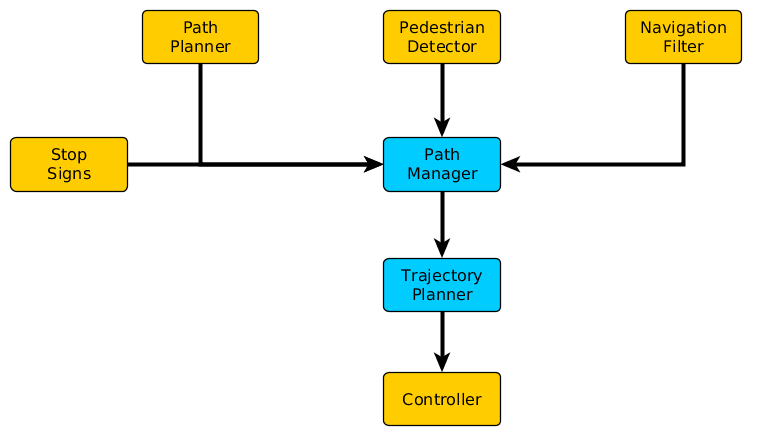
\includegraphics[width=1.0\columnwidth]{graphics/MissingReactionPiece2.png}
  \caption{Adding reactive behavior to trajectory planning}
  \label{fig:addreact}
\end{figure}
					


\section{Input Subsystems} \label{sec:inputsubsystems}

\begin{figure}[thpb]
  \centering
  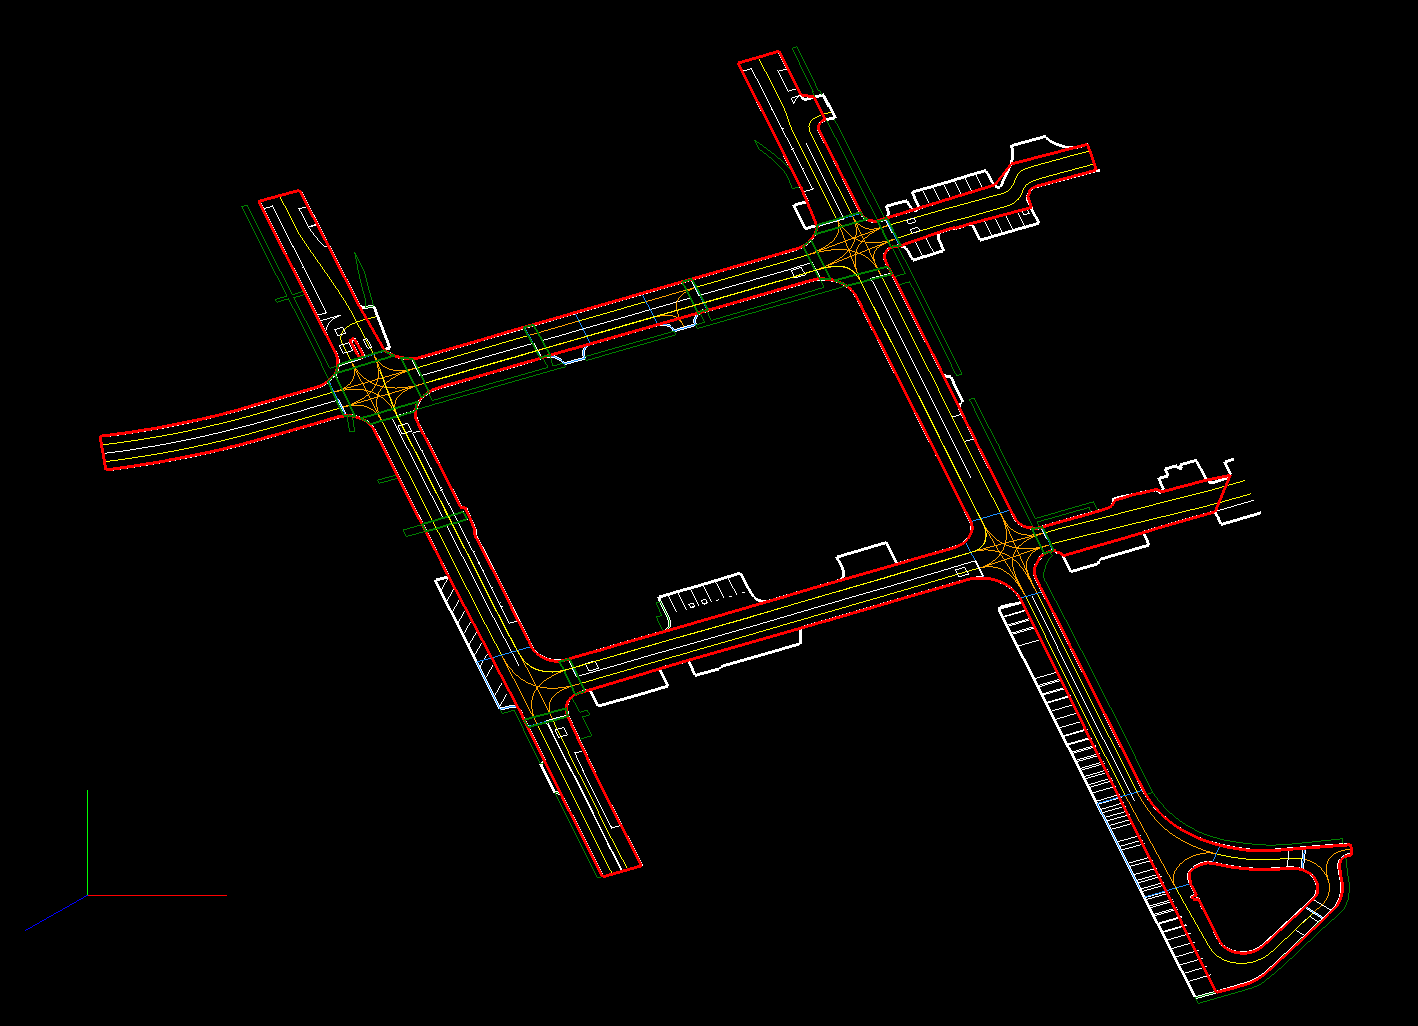
\includegraphics[width=1.0\columnwidth]{graphics/zenrin.png}
  \caption{High resolution map. Red color is at road edges. Green color shows lane center-lines}
  \label{fig:map}
\end{figure}

\begin{figure}[thpb]
  \centering
  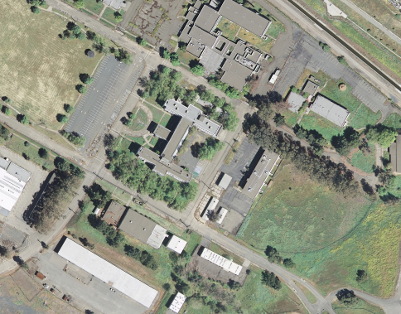
\includegraphics[width=1.0\columnwidth]{graphics/GoMentumSatelliteSmall.png}
  \caption{Gomentum map top view}
  \label{fig:gomentum}
\end{figure}

We assume that we have access to Path Planner. This can be for example a service similar to
Google Maps except that it provides lane level maps. We also assume that we have a High
Resolution digital map such as one shown in Figure \ref{fig:map} [corresponding to 
Figure \ref{fig:gomentum}] with Lane centers, Stop 
signs, crosswalk geometry, and Turning curves at intersections. The starting position the 
car is determined via high grade GPS. The destination is manually input into the system.
Using the path planner, we obtain a path along lane centers from start to the destination.
This plan is output as waypoints, with the waypoints corresponding to stop signs marked.

\begin{figure}[thpb]
  \centering
  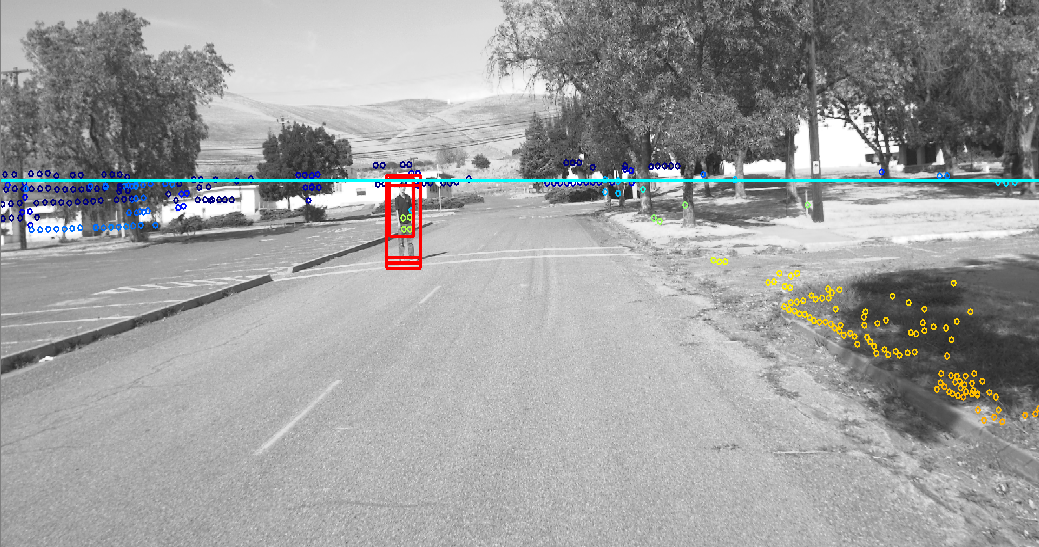
\includegraphics[width=1.0\columnwidth]{graphics/ped-detection-screenshot.png}
  \caption{Showing detected pedestrian by the computer vision system}
  \label{fig:ped}
\end{figure}

%\begin{figure}[thpb]
%  \centering
%  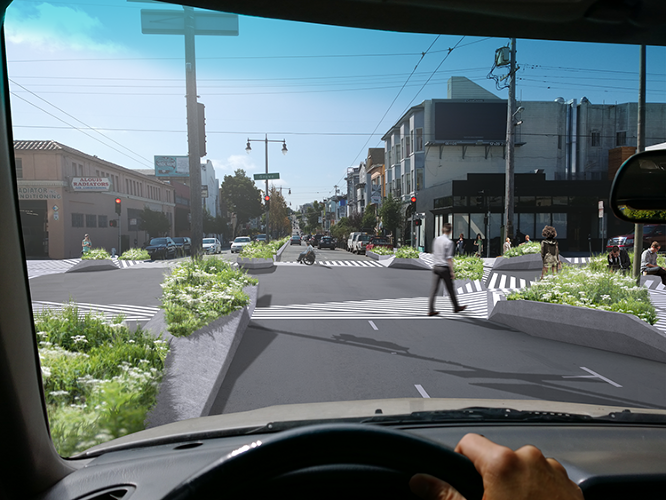
\includegraphics[width=1.0\columnwidth]{graphics/3023096-slide-c4carafter.png}
%  \caption{Pedestrain at the intersection}
%  \label{fig:ped2}
%\end{figure}

\begin{figure}[thpb]
  \centering
  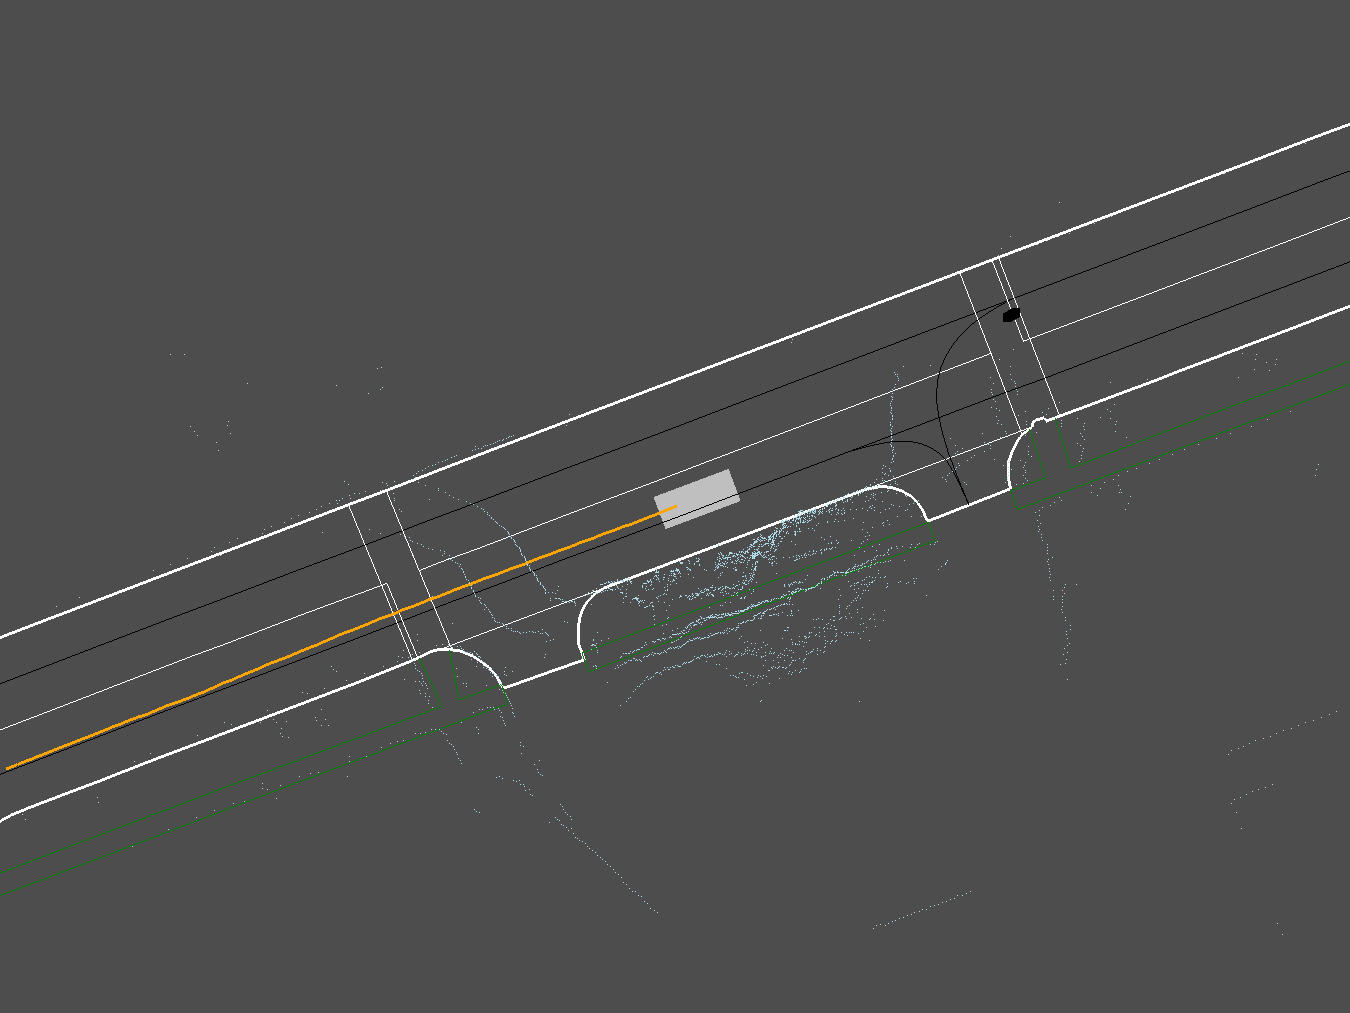
\includegraphics[width=1.0\columnwidth]{graphics/screenshot-objectmap.png}
  \caption{Showing car with road and path covered so far. The red filled circle shows the pedestrian for which the car is stopping}
  \label{fig:car}
\end{figure}

Pedestrian Detection is performed via a Camera, and LiDAR system. It computes a bounding 
box for each pedestrian as shown in Figure \ref{fig:ped}. The pedestrian position is 
transformed to the vehicle body frame, and subsequently transformed to global frame and 
can be shown on the map as in Figure \ref{fig:car}.

\begin{figure}[thpb]
  \centering
  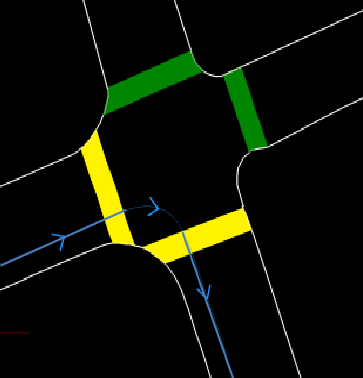
\includegraphics[width=0.5\columnwidth]{graphics/IntersectionCrosswalks.png}
  \caption{A car turning right at the intersection only needs to care about pedestrians in the 
pedestrian crossings shown yellow. Pedestrians in the green crossings can be ignored unless they
appear somewhere on the road}
  \label{fig:intersect}
\end{figure}

We also have an In-Out Algorithm implemented via polygon intersection that can be used to
ignore “safe” pedestrians that are on sidewalks, off-path crosswalks, and behind planned stop
as shown in Figure \ref{fig:intersect}.
Remaining pedestrians pose collision risk and we need to reactively slow down or stop for them.
This is accomplished by sending stop message with pedestrian locations to path manager.

For Navigation Filtering we use an ADMA-G based Commercial automotive GPS/INS system.
It receives RTK corrections via cell modem. It outputs Global position, global heading,
body frame velocity and body frame acceleration to 10s of cms.

\section{Path Manager} \label{sec:pathmanager}


Path Pre-processor conforms the path to planner assumptions. The Path Manager breaks up the
path at stop signs, decides when to stop, when to go and invokes the trajectory planner
as necessary. 

There are two types of stops - Planned (PSTOP) and Reactive (RSTOP). At reactive stops
to pedestrians, the car may slow down and restart if the pedestrian leaves before the
car comes to a stop; otherwise the car would come to a stop and restarts once the 
pedestrian leaves.

The state of the car is represented by a State Machine as shown in figure \ref{fig:st}

\begin{figure}[thpb]
  \centering
  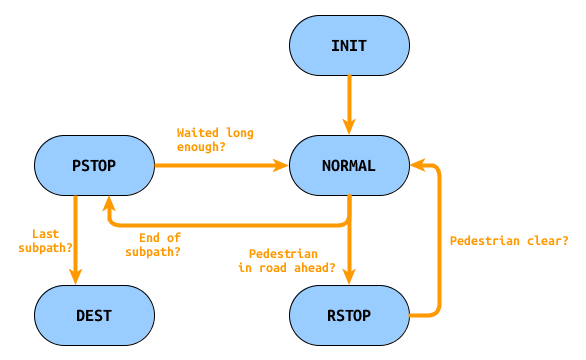
\includegraphics[width=1.0\columnwidth]{graphics/StateMachineSimple.png}
  \caption{State Transition Diagram}
  \label{fig:st}
\end{figure}


The assumption on our work is that there is a unique mapping from a time to s coordinate 
system. This mapping breaks down when we are stopped at a planned or reactive stop. 
The solution is to break the path into sub-paths, and plan and execute incrementally.
This is shown in Figures \ref{fig:segmentation} \ref{fig:stcur} and \ref{fig:scoord}.

\begin{figure}[thpb]
  \centering
  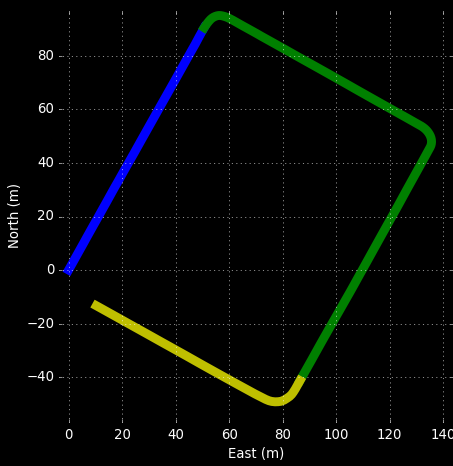
\includegraphics[width=0.5\columnwidth]{graphics/Subpaths.png}
  \caption{Segmentation of the path by path manager. The Trajectory generation is serially called on each segment colored differently. Need to update figure with stop signs????????????????}
  \label{fig:segmentation}
\end{figure}

\begin{figure}[thpb]
  \centering
  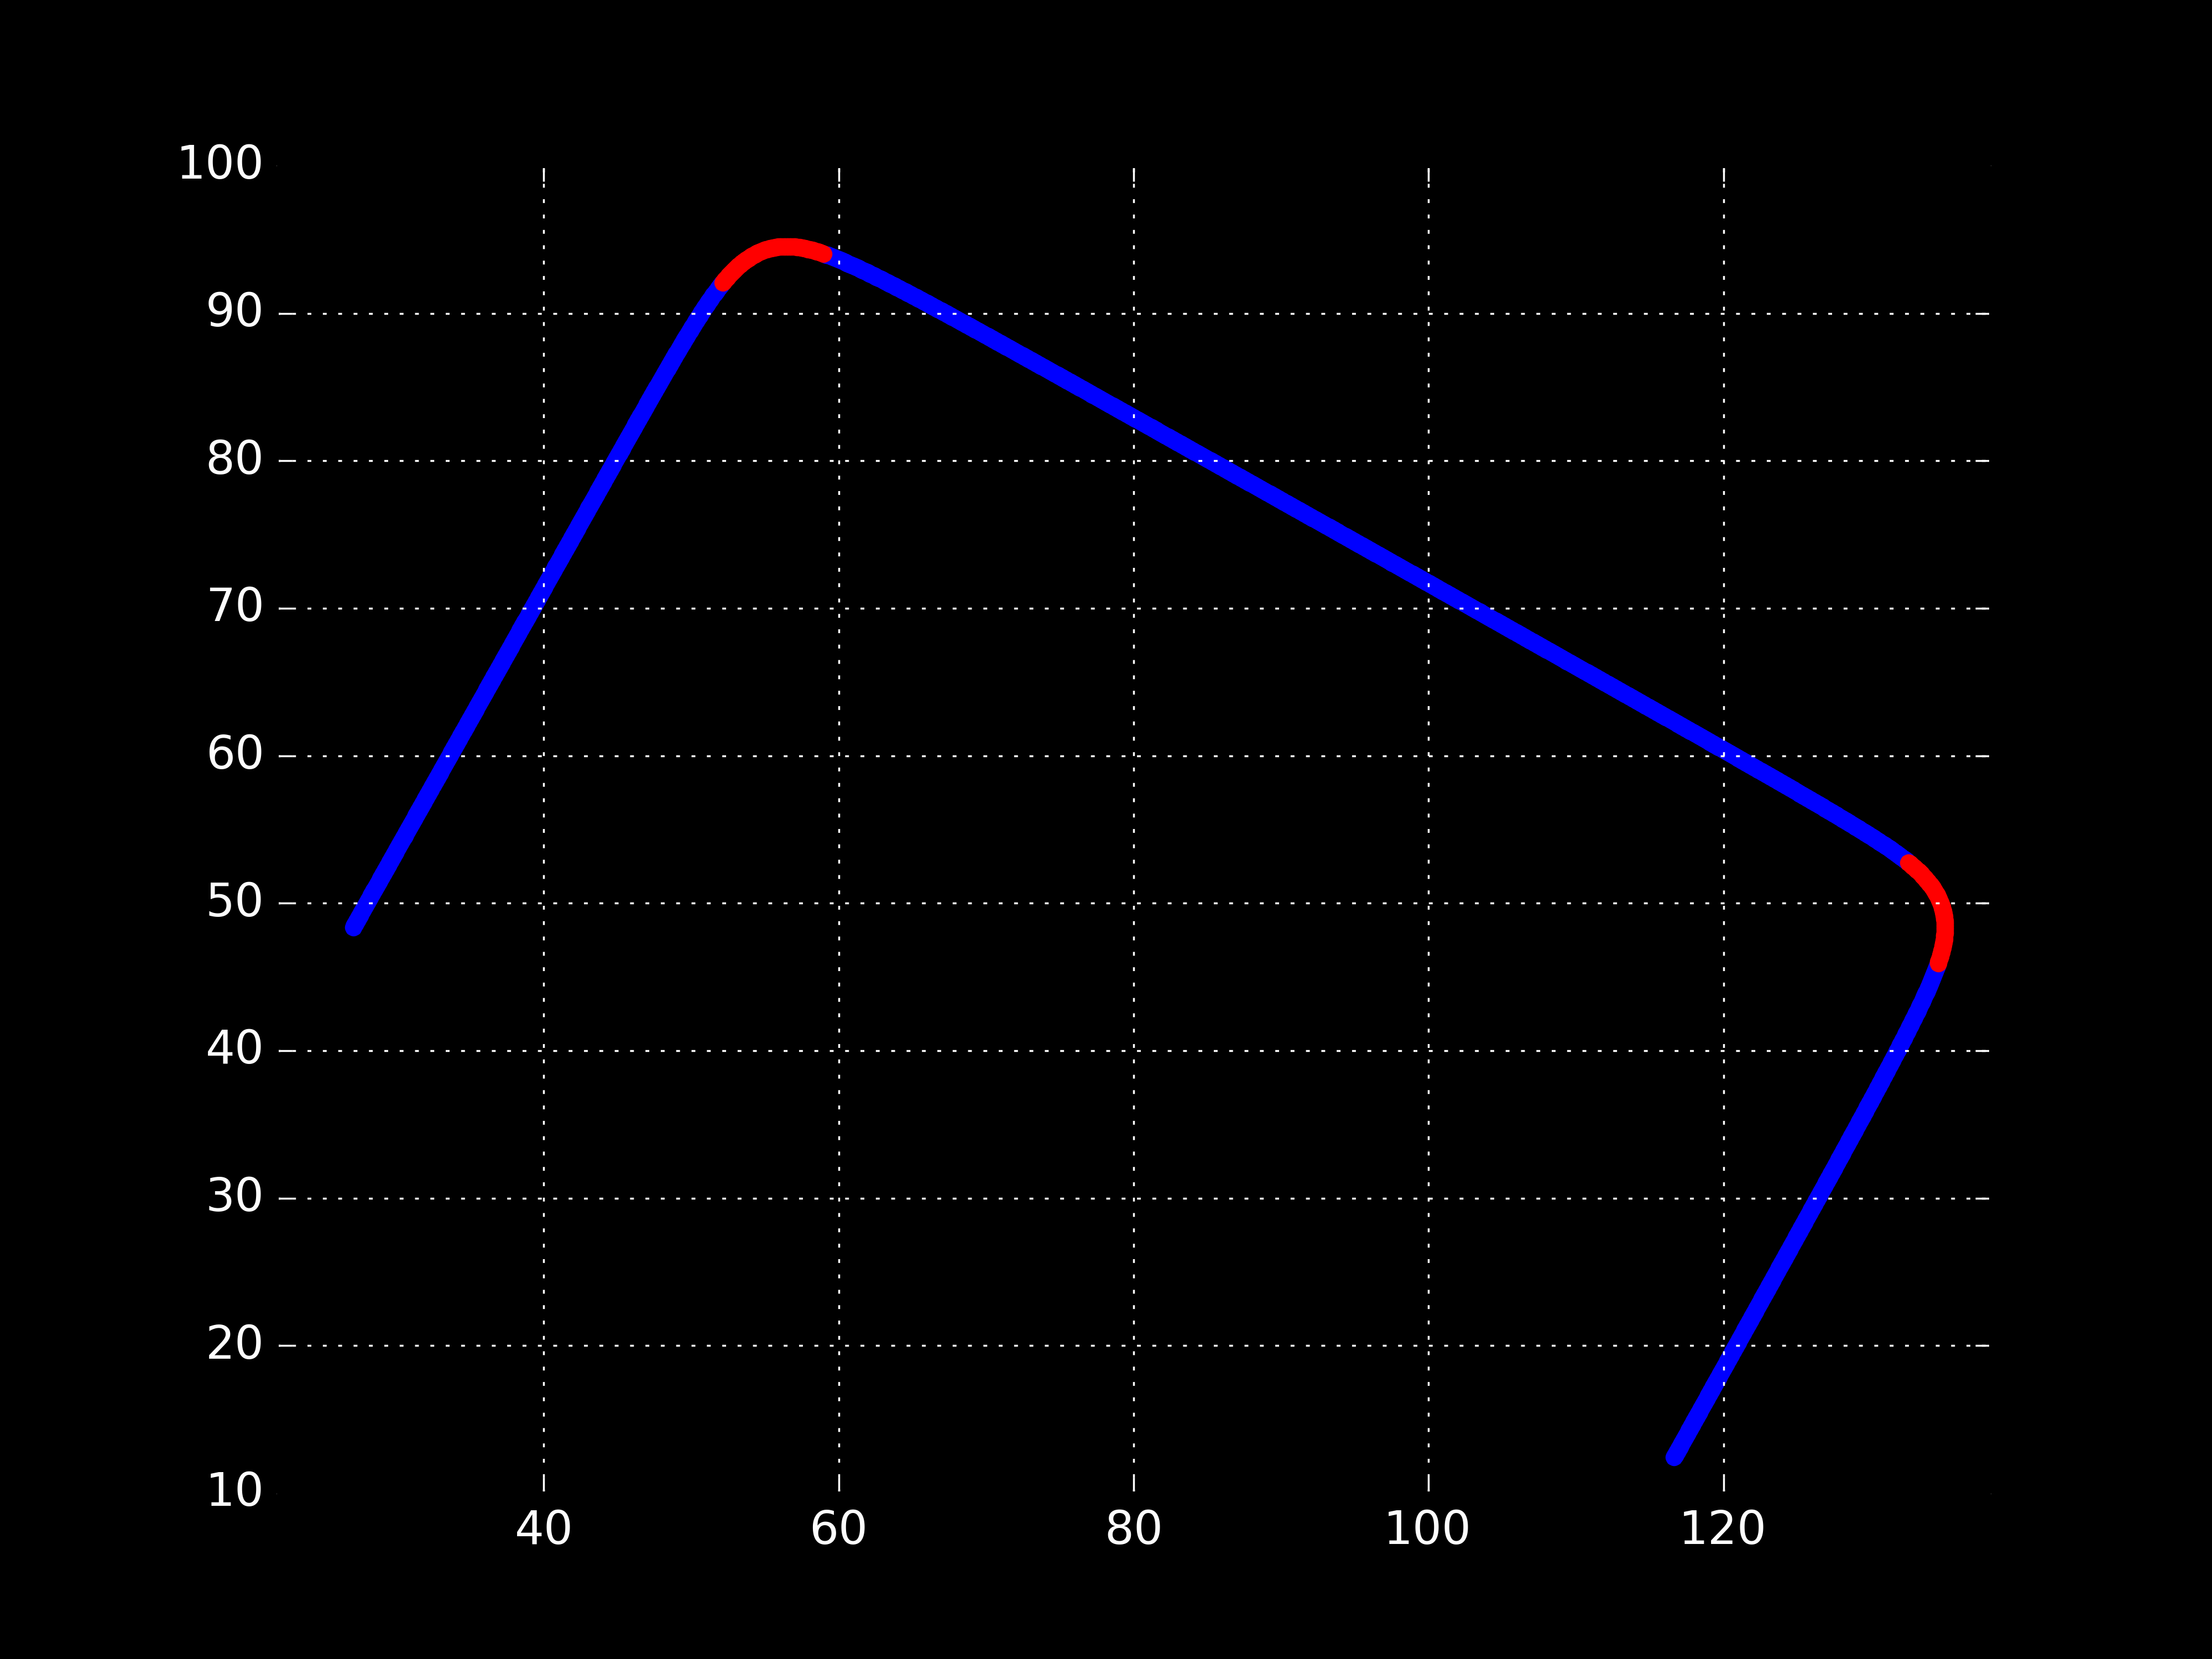
\includegraphics[width=0.5\columnwidth]{graphics/course_highlighted_turns.png}
  \caption{Further characterization of green path shown in segmentation figure into straight and curved parts}
  \label{fig:stcur}
\end{figure}

\begin{figure}[thpb]
  \centering
  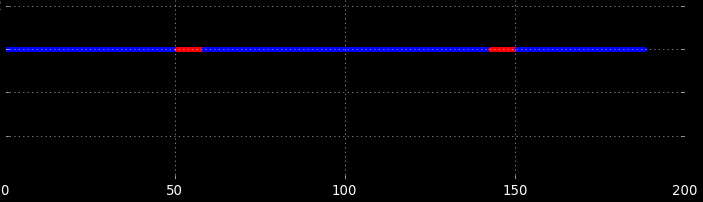
\includegraphics[width=1.0\columnwidth]{graphics/1Dsegmentation.png}
  \caption{Showing the path projected onto the one dimensional s coordinate system}
  \label{fig:scoord}
\end{figure}

The algorithm is:
\begin{itemize}
\item Send first sub-path to trajectory planner
\item Wait until completed
\item Pause for fixed time
\item Send next sub-path to planner
\item Repeat until end of path
\end{itemize}

For unplanned, reactive stops  we need to slow down and stop. There are three scenarios:
\begin{enumerate}
\item Normal pedestrian → appears
\item Stopping pedestrian → moves
\item Stopped pedestrian leaves →
\end{enumerate}

In the next section we describe when/where to begin braking, when/where to stop
and when to go again.

\section{Reactive Subsystem} \label{sec:reactiveubsystem}

\begin{figure}[thpb]
  \centering
  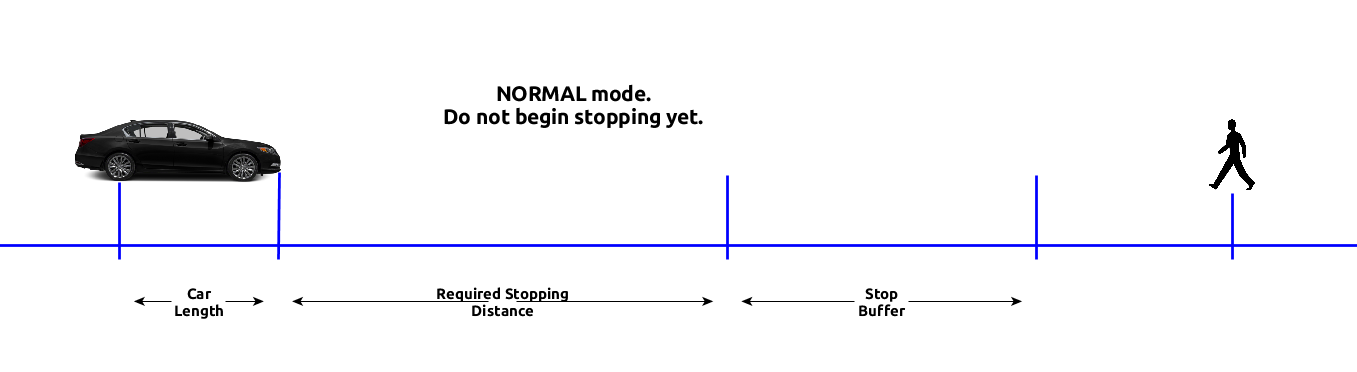
\includegraphics[width=1.0\columnwidth]{graphics/RSTOP_NORMAL.png}
  \caption{Normal mode}
  \label{fig:react1}
\end{figure}
\begin{figure}[thpb]
  \centering
  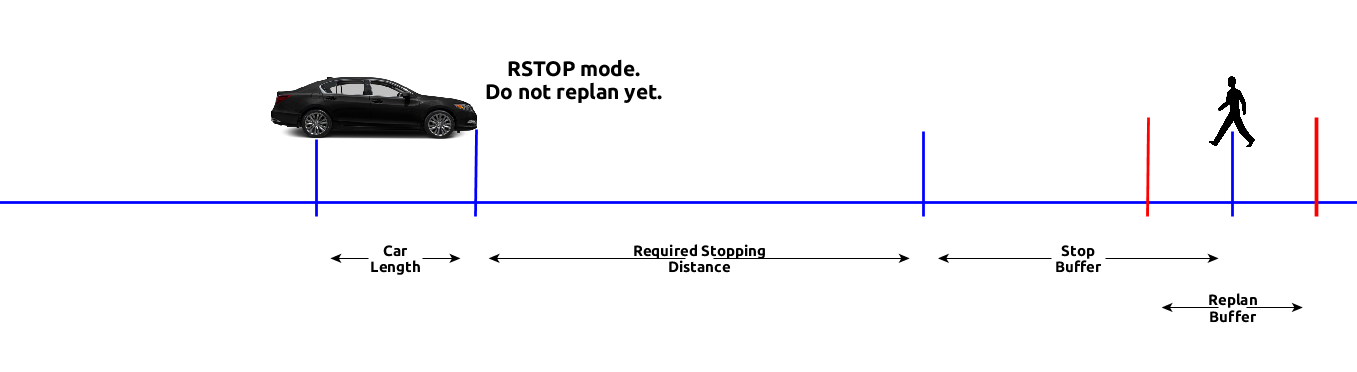
\includegraphics[width=1.0\columnwidth]{graphics/RSTOP_RSTOP.png}
  \caption{Stopping for the pedestrian mode}
  \label{fig:react2}
\end{figure}
\begin{figure}[thpb]
  \centering
  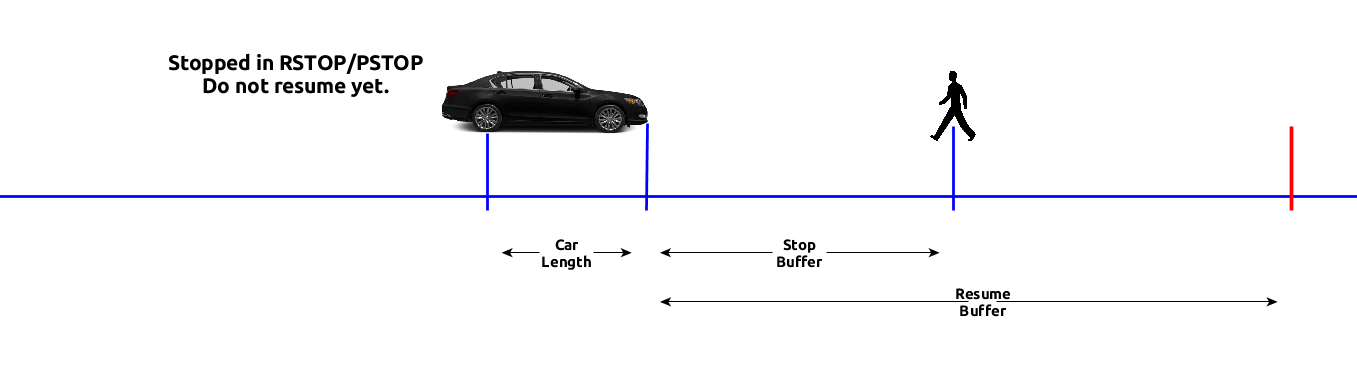
\includegraphics[width=1.0\columnwidth]{graphics/RSTOP_RESUME.png}
  \caption{Resuming after stop sign}
  \label{fig:react3}
\end{figure}



\begin{figure}[thpb]
  \centering
  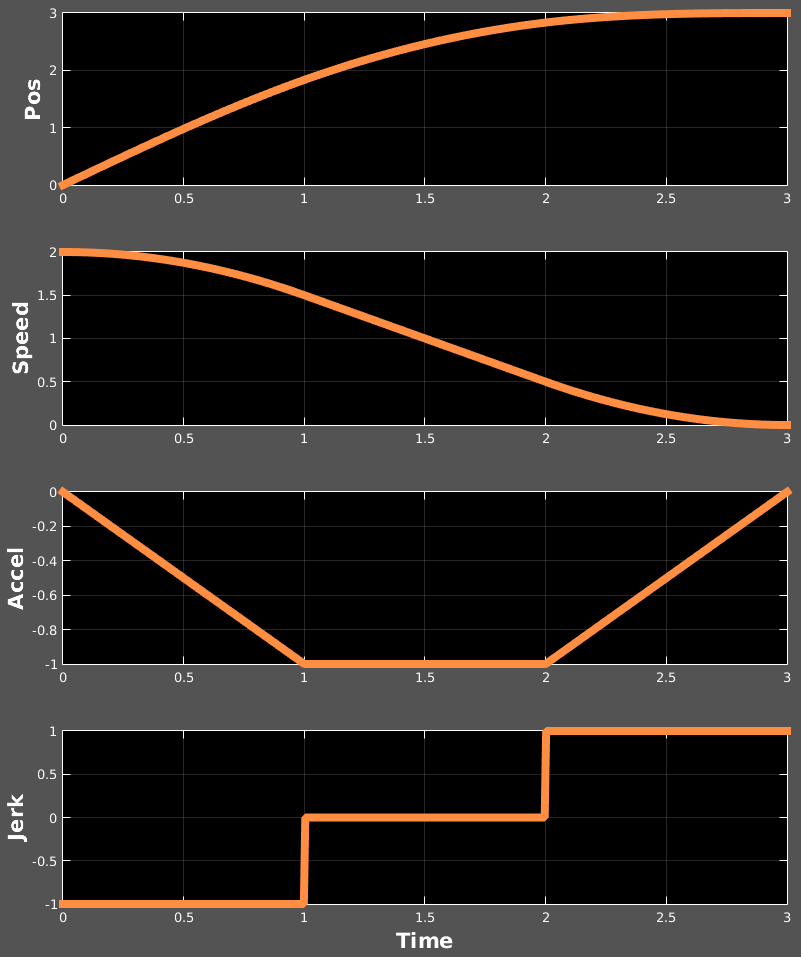
\includegraphics[width=1.0\columnwidth]{graphics/3phase_all_derivatives_SlowingDown.png}
  \caption{3 phase R stop}
  \label{fig:3phaserstop}
\end{figure}


\begin{figure}[thpb]
  \centering
  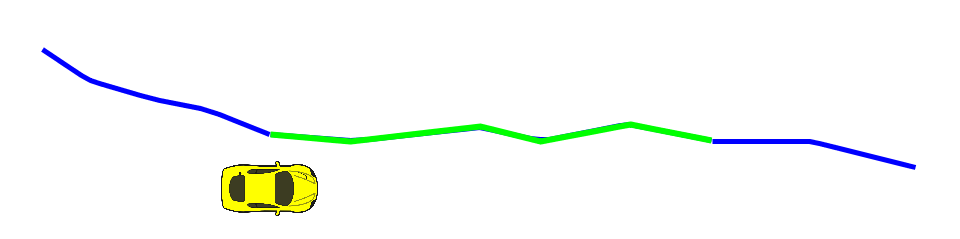
\includegraphics[width=1.0\columnwidth]{graphics/RSTOP_path_truncation.png}
  \caption{Green color path is the one over which the car finds a trajectory to stop}
  \label{fig:pathtostop}
\end{figure}


For reactive stopping, if there are multiple pedestrian ahead, we only consider the
closest pedestrian. That pedestrian is projected on the path of the car to determine the
required braking distance. The stopping trajectory is similar to rest of profile,
and consists of a single segment with 3 phases as shown in Figure \ref{fig:3phase}. 
The trajectory planner uses total distance as parameter, and is not suitable for
our purpose as the end speed constraints are not met. So we reformulate and 
replace $L$ with $v_f$ as hard constraint.

Typically while with the Trajectory Planner, we get initial conditions from the
navigation filter. We use normal (sedate) peak parameters for acceleration
and jerk. We plan a 3 phase stop profile with the current required stopping distance.

Once a pedestrian enters the stop zone, we need to plan, and execute RSTOP trajectory.
When available distance <= “required” distance, we increase acceleration, jerk peaks to
match available distance.

After a reactive stop we split the path before the stop from the one after the stop
sign and execute the later as a separate trajectory. The plan is stored and sampled 
the same as in normal operation.

To get back to normal driving after we are fully stopped, we resume
after pedestrian leaves roadway, or pedestrian moves far down roadway.
When he moved further down, we stop again later after we are a threshold
distance away. The effect is that we follow the person at the distance with some 
delay in chunks of few meters each time. If the pedestrian leaves before 
the car comes to a full stop, the car can speed up without stopping using the 
same algorithm.


\section{Summary} \label{sec:summary}

We have built a robust stopping model as part of Trajectory planner reliably integrated with path manager.
We can travel along desired path, stop at stop signs, stop for pedestrians in roadway, and continue after 
they leave. Our system handles corner cases gracefully, and works with multiple pedestrians as we only 
need to consider the closest pedestrian ahead of us. In future, we want to handle other roadway traffic, 
coexisting with other vehicles. We would also like to perceive and stop for red-lights.

\section{Examples}

\begin{figure}[thpb]
  \centering
  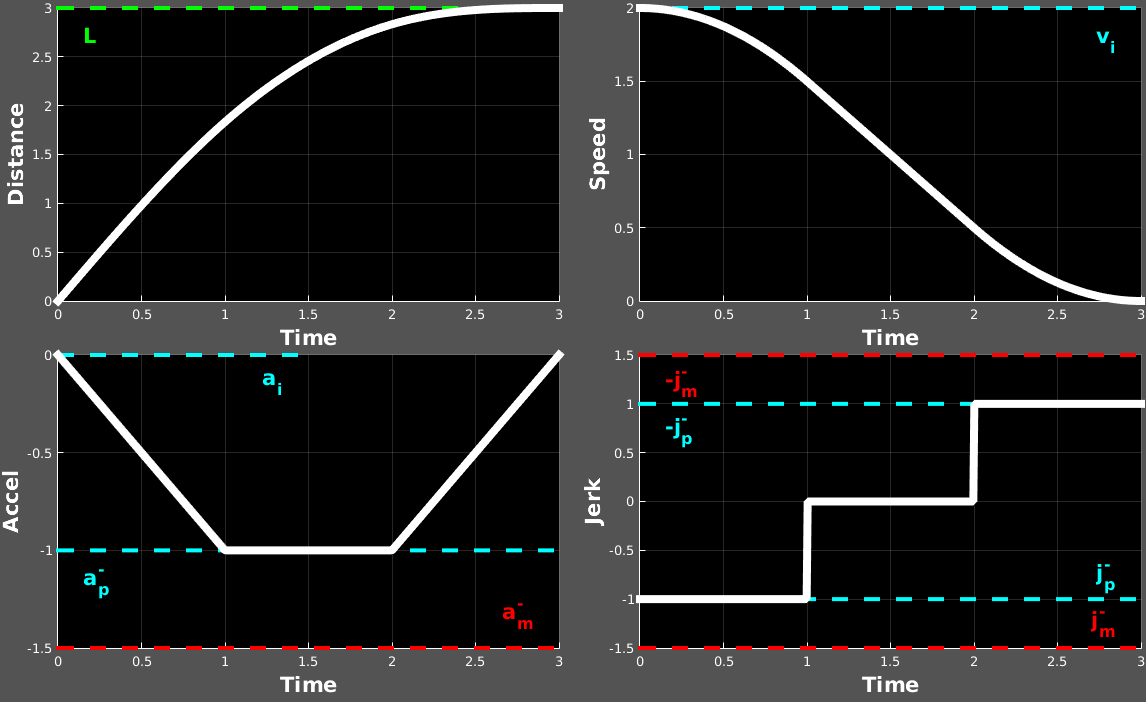
\includegraphics[width=1.0\columnwidth]{graphics/FullStopSpec.png}
  \caption{Example 3 phase jerk profile}
  \label{fig:3phase}
\end{figure}

\section{2d to 1d conversion}


\begin{figure}[thpb]
  \centering
  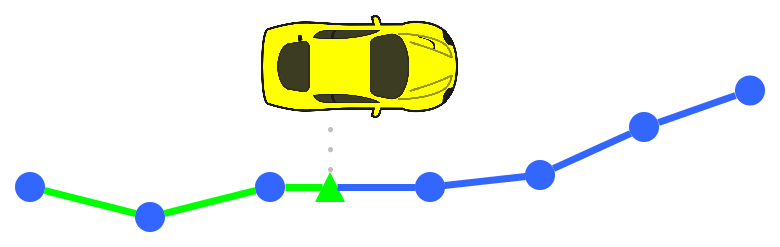
\includegraphics[width=0.5\columnwidth]{graphics/PathProjection.png}
  \caption{Showing projection of current position of car shown by green triangle to s coordinate system}
  \label{fig:cartos}
\end{figure}
\begin{figure}[thpb]
  \centering
  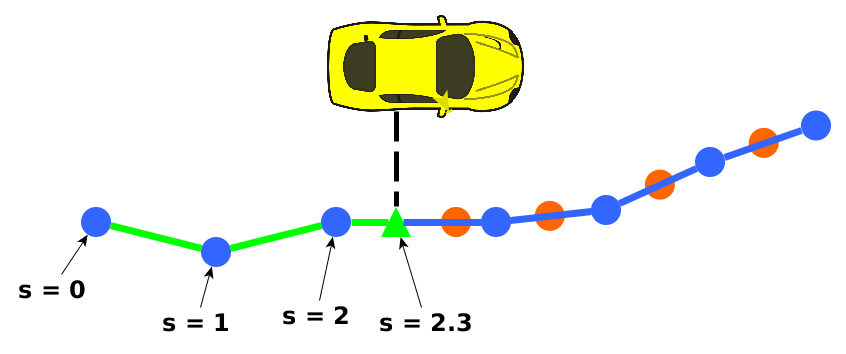
\includegraphics[width=0.5\columnwidth]{graphics/PathProjectionSlice.png}
  \caption{car to s coord with additional points}
  \label{fig:cartos2}
\end{figure}
\begin{figure}[thpb]
  \centering
  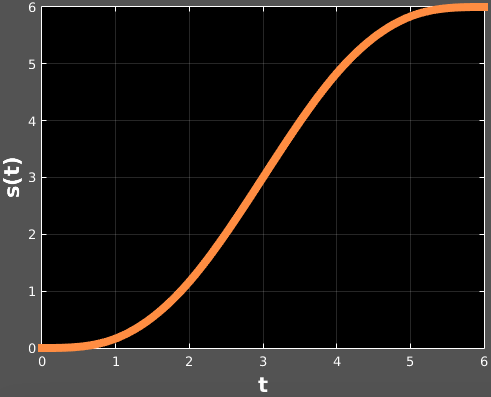
\includegraphics[width=0.5\columnwidth]{graphics/s(t)_generic.png}
  \caption{Transformation from s coordinate system to time}
  \label{fig:stot}
\end{figure}

\section{Other Issues}
                
\begin{figure}[thpb]
  \centering
  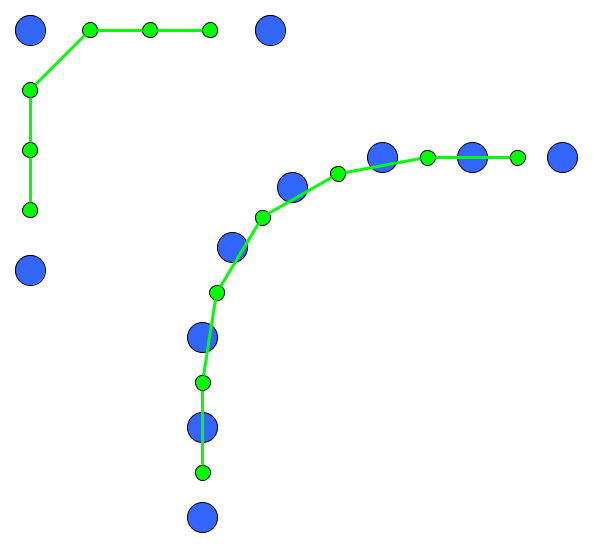
\includegraphics[width=0.5\columnwidth]{graphics/LowResPathSample.png}
  \caption{Grid discretization issue}
  \label{fig:discretization}
\end{figure}
\begin{figure}[thpb]
  \centering
  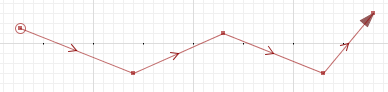
\includegraphics[width=0.5\columnwidth]{graphics/linestring.png}
  \caption{Exaggerated view of path points which may have discontinuous curvature}
  \label{fig:disc}
\end{figure}

\begin{figure}[thpb]
  \centering
  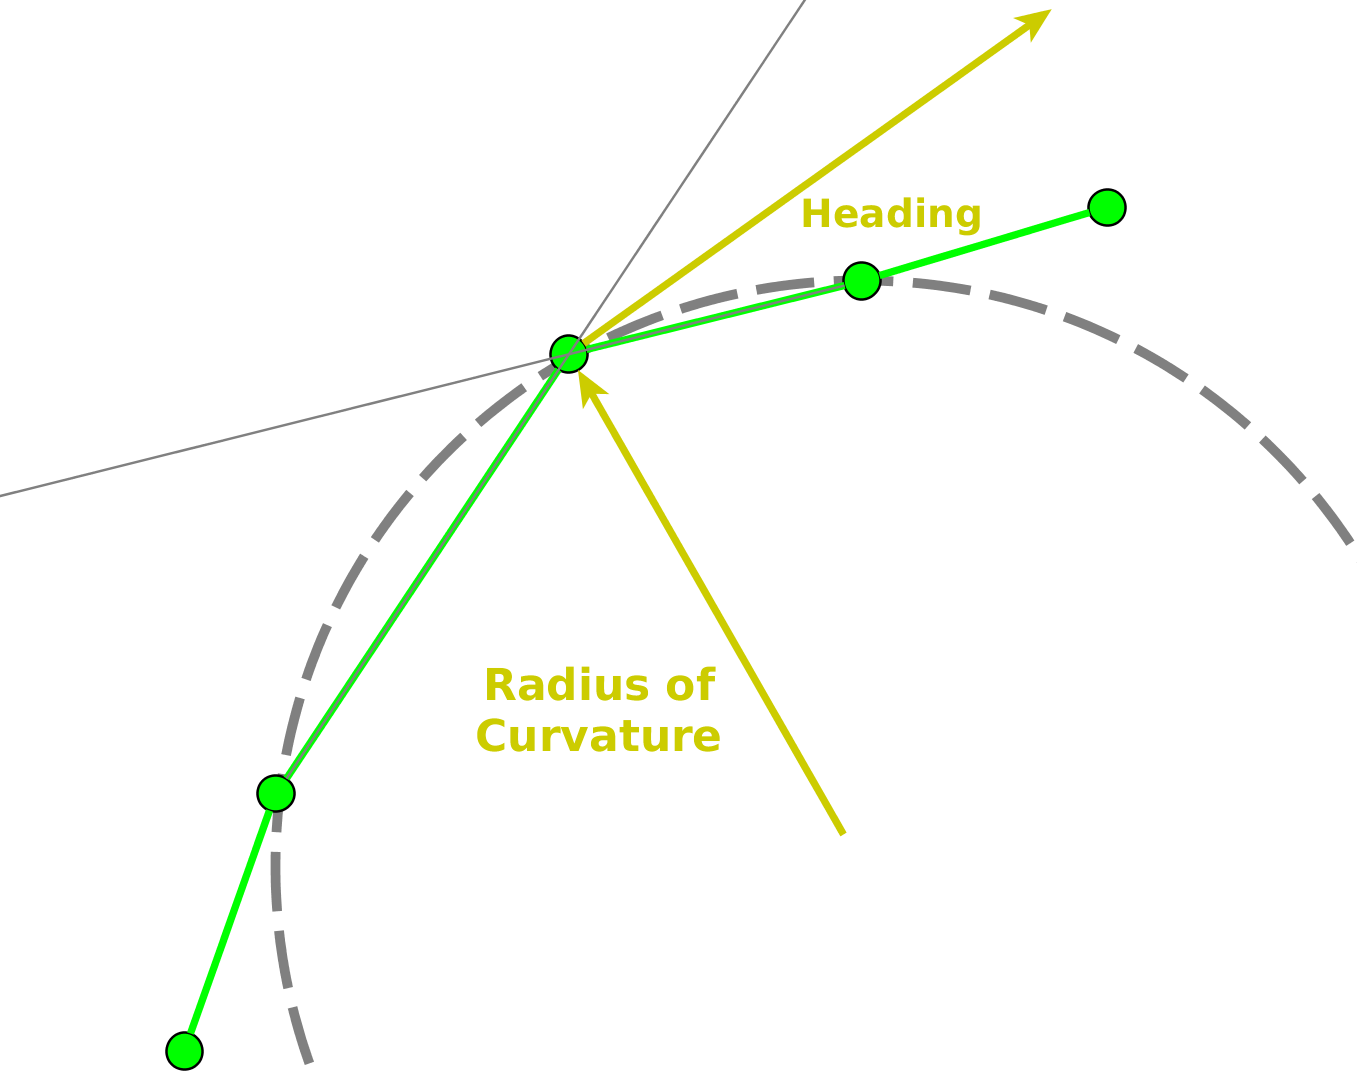
\includegraphics[width=0.5\columnwidth]{graphics/CircularCurvature.png}
  \caption{circular curvature}
  \label{fig:curv}
\end{figure}

\begin{figure}[thpb]
  \centering
  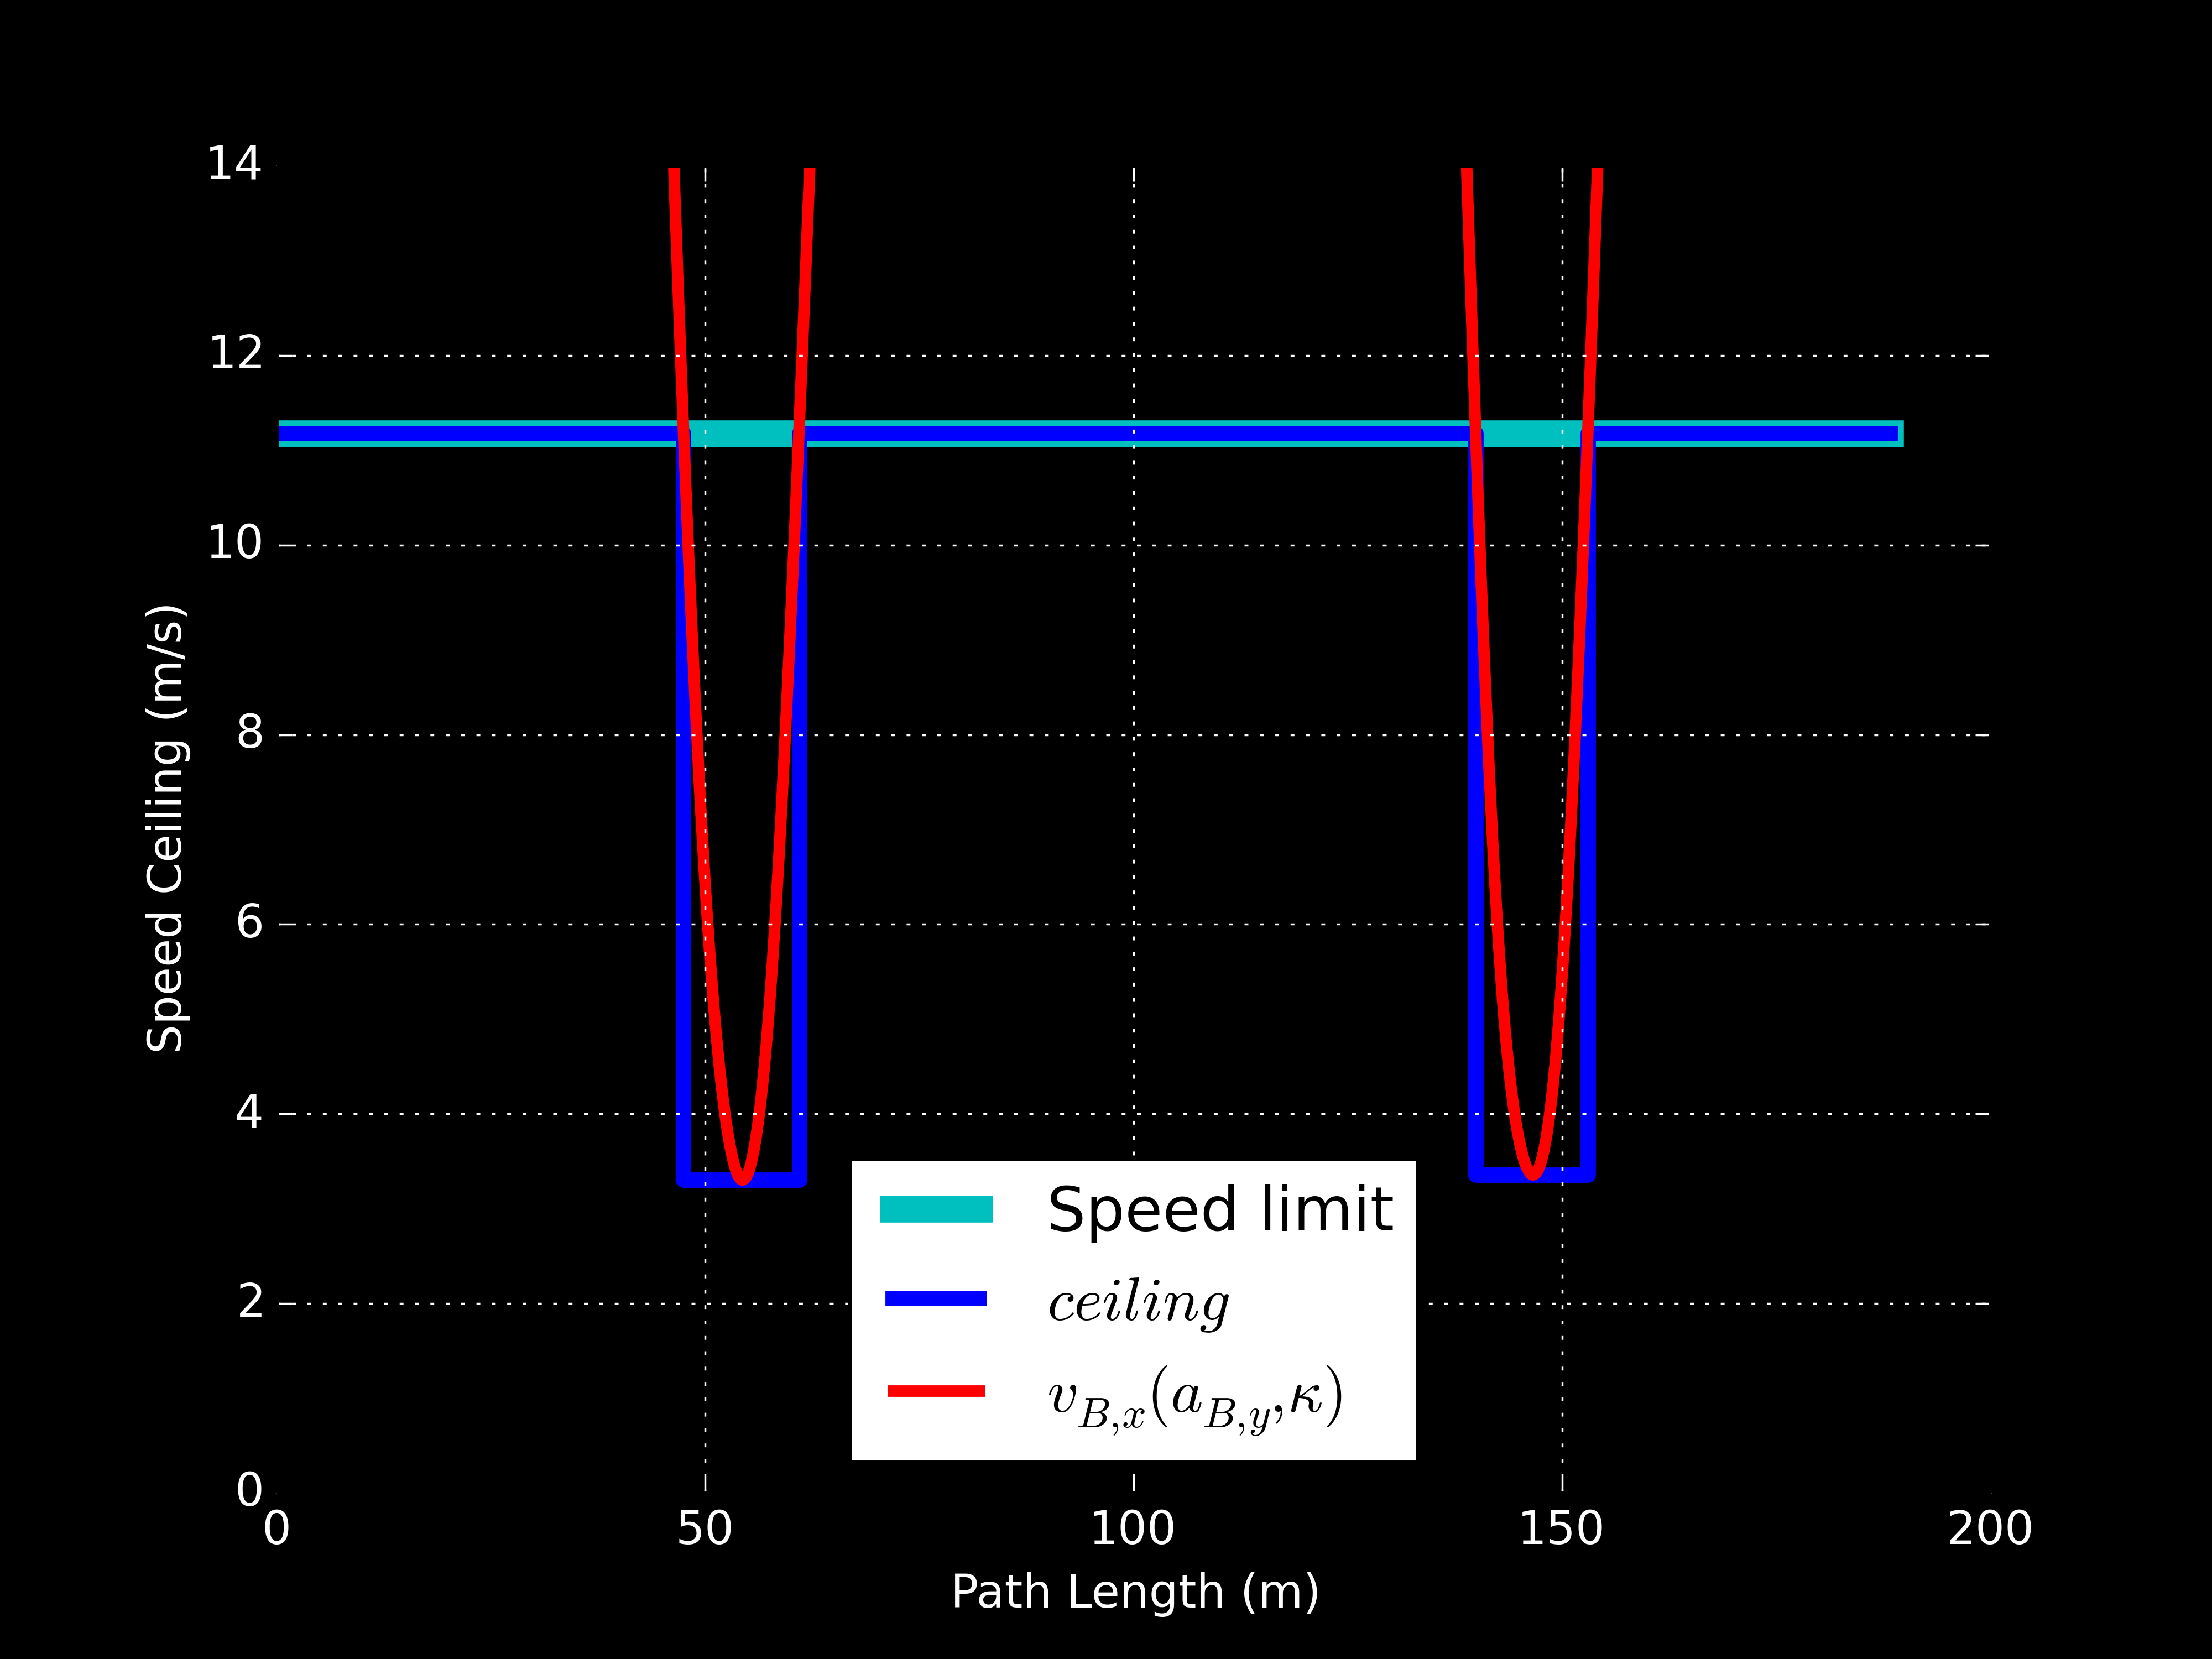
\includegraphics[width=0.5\columnwidth]{graphics/speed_ceiling.png}
  \caption{Speed Ceiling}
  \label{fig:speedceil}
\end{figure}

\begin{figure}[thpb]
  \centering
  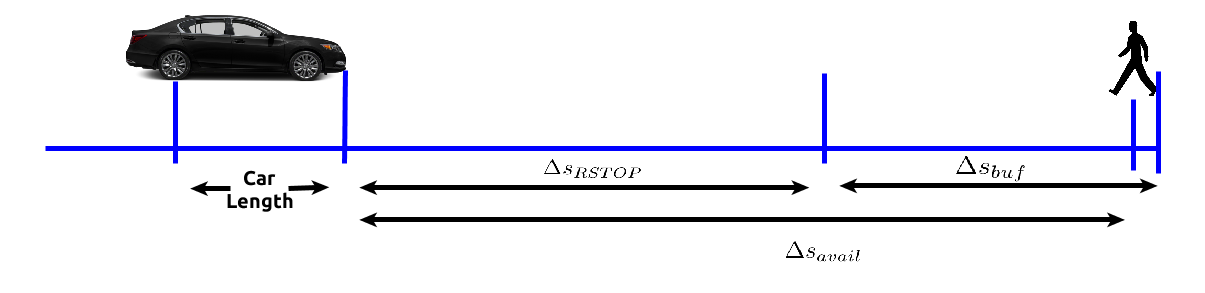
\includegraphics[width=1.0\columnwidth]{graphics/RSTOP_NORMAL_time_to_stop.png}
  \caption{Reaction Response: Normal Mode}
  \label{fig:7phaseprofile}
\end{figure}



           
\section{Implementation}

\emph{How much should we say here?}

\section*{Acknowledgments}

Thanks...

%%%%%%%%%%%%%%%%%%%%%%%%%%%%%%%%%%%%%%%%%%%%%%%%%%%%%%%%%%%%%%%%%%%%%%%%%%%%%%%%

\bibliographystyle{IEEEtran}
\bibliography{HRI_internship_trajectory_planner_articles}

\end{document}




